\section{Double resonance}
\subsection{Set-up and procedure}
\begin{figure}[htb]
\centering
\includegraphics[width=1.0\linewidth]{graphics/doubleresonancesetup}
\caption[Double resonance set-up]{Experimental set-up for the double resonance measurements.\cite{anleitung}}
\label{fig:doubleresonancesetup}
\end{figure}
This measurement is called double resonance since both pump the Zeeman states are pumped and, at the same time, the polarized state is de-popularized with radio frequency radiation (RF radiation from here on). Both effects can be described as a resonance. The RF frequency can be measured with a frequency counter which is also built into the glass cell unit.  The glass cell is now always lodged in the central unit.\\
To achieve pumping, the polarization of the laser light needs to be changed from linear to circular. It does not matter whether it is right or left circular - that merely changes the direction of polarization. To achieve circular polarization, a quarter wave plate is used. As the polarization after said place depends on the angle of the linear polarization of the incident light relative to the relevant crystal axis, one has to check whether the light is actually circularly polarized after the wave plate. For that, a linear polarizer is used to check whether or not the intensity signal varies upon turning the linear polarizer, which it should not.\\ 
A sinusoid current is run through coil 2 (see fig. \ref{fig:doubleresonancesetup}), at first with a large amplitude to find the magnetic field range for which double resonance occurs. Once the range is determined, a constant current is applied to coil 1. The double resonance peaks are now visible, but Dehmelt peaks, which are a result of relaxation once the magnetic field crosses zero, are still visible. It can easily be determined which is which, as the double resonance peaks disappear when one turns off the RF generator. For the Dehmelt peaks to disappear, the amplitude of the sinusoid in current two has to be reduced so that the overall magnetic field does not cross zero anymore.  Coil 4, which creates a field along the x-axis in figure \ref{fig:doubleresonancesetup}, can now be used to compensate the vertical magnetic field of the earth. When it is compensated, the negative peaks should have maximal depths. The current through coil 4 is then kept at this value for the main measurement.\\
With the vertical magnetic field compensated, the current in coil 1 can now be tuned to make the two peaks per period of the signal in coil 2 equidistant. In this state, the magnetic field from coil 1 stretches the Zeeman spectrum exactly enough for the RF frequency to relax the polarization. One such value must exist for both current directions through coil 1. This is done for both rubidium isotopes. The current in coil 1 is measured with an exterior multimeter, since the digital display only has a precision of $\unit{1}{mA}$. From these four values, the longitudinal magnetic field of the earth can be measured and the nuclear spins $I$ of the isotopes calculated.

\subsection{Data analysis}
\begin{figure}
\centering
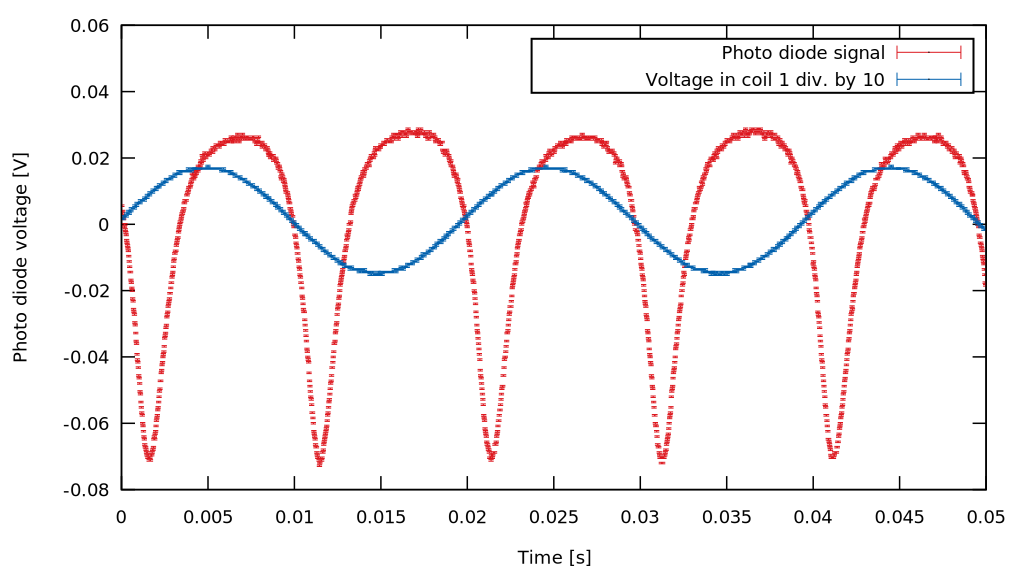
\includegraphics[width=1.0\linewidth]{graphics/equaldistance}
\caption[Double resonance peaks]{Equidistant peaks for $I_L=\unit{61.8}{mA}$ and a current in coil 1 of $I_{C1}=\unit{130.2}{mA}$. Note the phase shift: The double resonance peaks do not occur at the zero-crossing of the coil voltage, but at those of the coil current. The coil voltage was divided by ten to make the photo diode signal more dominant.}
\label{fig:equaldistance}
\end{figure}
Measurements were taken at $T=\unit{34.4}{\degree}$ and for a RF frequency of $\nu_{RF}=\unit{(497\pm1)}{kHz}$. An uncertainty of $s_{I_{C1}}=\unit{0.5}{mA}$ was estimated for current at which the peaks are equidistant. The results can be seen in table \ref{tb:doubleresonance}. The current in coil 4 for which the vertical field was compensated was determined to be $I_{C4}=\unit{(78\pm3)}{mA}$.\\
The constants $c_B=B/I$ of the coils in table \ref{tb:coilconstants} were provided \cite{anleitung} for the calculations of the magnetic fields that the coils create.

\begin{table}\centering
	\begin{tabular}{@{}llllll@{}}
		\toprule
		&Coil No&n &d [m]&calc. $\unit{B/I}{[\frac{Vs}{Am^2}]}$&meas. $\unit{B/I}{[\frac{Vs}{Am^2}]}$]\\ 
		\midrule
		&1&80&0.09&$8.0\cdot10^{-4}$&$7.99(1)\cdot10^{-4}$\\
		&2&80&0.09&$8.0\cdot10^{-4}$&$8.14(1)\cdot10^{-4}$\\
		&3&16&0.09&$1.7\cdot10^{-4}$&--\\
		&4&60&0.246&$4.4\cdot10^{-4}$&$4.76(1)\cdot10^{-4}$\\
		\bottomrule
	\end{tabular}
	\caption[Properties of the magnetic field coils]{The $B/I$ values and properties of the Helmholtz coils. $n$ is the number of windings. \cite{anleitung}}
	\label{tb:coilconstants}
\end{table}
The magnetic fields are
\begin{equation}
B=c_b\cdot I_C,\qquad s_B=\sqrt{(c_b\cdot s_{I_C})^2+(I_C\cdot s_{c_b})^2}
\end{equation}
where $I_C$ is the current in the respective coil. Table \ref{tb:doubleresonance} lists those results for coil 1.\\ From the current in coil 4, the vertical magnetic field was calculated to be
\begin{equation}
B_v=\unit{(37.1\pm1.4)}{\micro T}
\end{equation}
\begin{table}\centering
	\begin{tabular}{@{}lllllll@{}}
		\toprule
		&$I_L$ [mA]&$s_{I_L}$ [mA]&$I_{C1}$	[mA]&$s_{I_{C1}}$ [mA]&$B_{C1}$ [\micro T]&$s_{B_{C1}}$ [\micro T]\\ 
		\midrule
		&62.4&0.1&91.2&0.5&71&10\\
		&62.4&0.1&-85.3&0.5&85&9\\
		&61.8&0.1&136.1&0.5&109&12\\
		&61.8&0.1&-130.2&0.5&104&11\\
		\bottomrule
	\end{tabular}
	\caption[Results of the double resonance measurements]{The results of the double resonance measurements. The magnetic field signs were matched with those of the currents.}
	\label{tb:doubleresonance}
\end{table}
The magnetic fields are all written with a positive sign. Let $B_1$ be the magnetic field of the positive, $B_1'$ the negative coil current. The horizontal component of the earths' magnetic field is equal to half the difference of these two fields
\begin{equation}
B_h=\frac{B_1-B_1'}{2},\qquad s_{B_h}=\frac{1}{2}\cdot\sqrt{s_{B_1}^2+s_{B_1'}^2}
\end{equation}
The magnetic field difference is identical for the two isotopes, but the error is slightly different. The mean of the two is
\begin{equation}
B_h=\unit{(2.36\pm 0.21)}{\micro T}
\end{equation}
When calculating the mean value of $B_1$ and $B_1'$,
\begin{equation}
\overline{B}_1=\frac{B_1+B_1'}{2}
\end{equation}
the magnetic field component of the earth cancels out and yields the magnetic field that is responsible for the Zeeman splitting. Together with the frequency $\nu_{RF}$ and by using equation \ref{eq:zeemanlevels}, the nuclear spins $I$ of the two isotopes can be calculated as
\begin{equation}
I=\frac{\mu_B\cdot \overline{B}_1}{h\cdot\nu}-\frac{1}{2},\qquad s_I=\frac{\mu_B\cdot \overline{B}_1}{h\cdot\mu}
\sqrt{\left(\frac{s_{\overline{B}_1}}{\overline{B}_1}\right)^2
	+\left(\frac{s_\nu}{\nu}\right)^2}
\end{equation}
Since greater diode current corresponds to lower frequency and thus lower transition energy, the current $I_{C1}=\unit{62.4(1)}{mA}$ corresponds to $^{87}$Rb and the $I_{C1}=\unit{61.8(1)}{mA}$ to $^{85}$Rb. The results for the spins were
\begin{align}
	I(^{85}\text{Rb})&=2.496\pm0.009\\
	I(^{87}\text{Rb})&=1.486\pm0.007\\
\end{align}
\subsection{Discussion}
The literature values for the earths' magnetic field are \cite{anleitung}
\begin{equation}
B_v^{lit}=\unit{42.9}{\micro T}, \quad B_h^{lit}=\unit{20.9}{\micro T}
\end{equation}
and the measurements yielded $B_h=\unit{(2.36\pm 0.21)}{\micro T}$ and $B_v=\unit{(37.1\pm1.4)}{\micro T}$. While the result for the vertical field encloses the literature value in its $4\sigma$ interval, the result for the horizontal field is nowhere near the expected value. To double check the results, a Hall effect sensor was used. Since the sensor only had a resolution of $\unit{10}{\micro T}$, it was only useful for a qualitative analysis. These measurements (see appendix) revealed that not only is the horizontal field much weaker inside the metal casing of the experimental set-up, the experimental set-up is also not aligned with the projection of the magnetic field lines on its horizontal axis. Due to time constraints, the measurements could not be repeated with an aligned table. The deviation in the vertical field can likely be attributed to shielding effects of the building.\\

The calculated values for the spins are in good agreement, enclosing the expected values of $I(^{87}Rb)=\nicefrac{3}{2}$ in the $2\sigma$ interval and $I(^{85}Rb)=\nicefrac{5}{2}$ in the $1\sigma$ interval.
